\chapter{Конструкторский раздел}
\label{cha:design}
\section{Общая архитектура приложения}
\begin{figure}[h!]
	\centering
	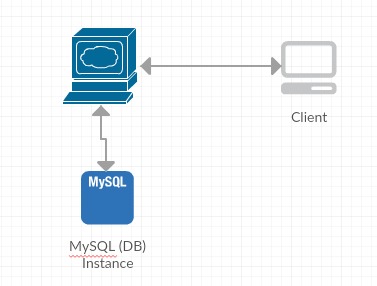
\includegraphics[width=0.6\textwidth]{img/img5.png}
	\caption{Общая архитектура приложения}
	\label{fig:spire09}
\end{figure}
Приложение построено по архитектуре "клиент-сервер". Клиент запускает на своём компьютере приложение и взаимодействует посредством сети с удаленным сервером. Сервер позволяет осуществлять доступ к необходимой информации из базы данных, разграничивать доступ пользователей к той или иной информации. Так же на сервере находится приложение, позволяющее парсить trace-файлы программы и заносить информацию в базу данных.
)

\section{Клиентская часть}
Клиентское приложение позволяет осуществлять авторизацию, получать информацию о доступном ему списке файлов трасс, получать общую информацию о файле трасс, получать детальную информацию о файле трасс в заданном временом временном интервале с заданным количеством процессов.
\begin{figure}[h!]
	\centering
	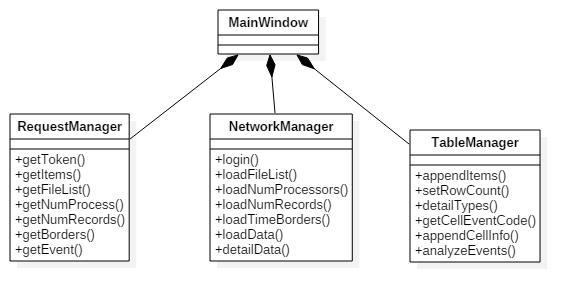
\includegraphics[width=0.8\textwidth]{img/client.png}
	\caption{Диаграмма классов клиентского приложения}
	\label{fig:spire10}
\end{figure}
\\ \textbf{MainWindow.} Класс графического интерфейса приложение. Реализует логику взаимодействия между клиентом и программой.\\
\textbf{NetworkManager.} Класс работы с сетью. Реализует логику асинхронных запросов к серверу.\\
\textbf{RequestManager.} Класс работы с телами ответов сервера.Парсит приходяющую с сервера информацию. \\
\textbf{TableManager.} Класс работы с визуалиацией приходящей информации. Реализует логику работы с таблицей отображения trace-информации.
\section{Серверная часть}
Сервер был разработан на базе NodeJS express. Он позволяет асинхронно работать с поступающим ему запросами. Код сервера представляет собой множество функций-обработчиков приходящих запросов.
\begin{lstlisting}[language=c++]
apiRoutes.get('/authenticate', function (req, res) {..}
apiRoutes.get("/getFile", function (req, res) {...}
apiRoutes.get("/getTimeBorders", function (req, res) {...}
apiRoutes.get("/getFileList", function (req, res) {...}
apiRoutes.get("/getNumRecords", function (req, res) {...}
apiRoutes.get("/getCodeInfo", function (req, res) {...}
apiRoutes.get("/getNumProcesses", function (req, res) {...}
\end{lstlisting}

\subsection{API для взаимодействия с сервером}
Была разработано API взаимодействия между клиентом и сервером. Безопастность взаимодействия гарантируется тем, что взаимодействия осуществляется на основе токенов. Все запросы, кроме запроса на авторизацию, требуют содержания в себе уникального токена.Токен дается клиенту после успешного прохождения авторизации. 
\begin{lstlisting}[language=c++]
(*\bfseries [GET] /authenticate *)
Авторизация
Аргументы
)name - логин
)password - пароль

(*\bfseries [Example response]*)
{
"success": true,
"message": "Enjoy your token!",
"token": "eyJhbGciOiJIUzI1NiIsInR5cCI6IkpXVCJ9.eyJ1c2VyIj
oiVXNlciIsInBhc3N3b3JkIjoicHdkI
iwiaWF0IjoxNDk2NDM4ODc4LCJleHAiOjE0OT
Y1MjUyNzh9.0bhg6Ct8YXOGixVY-ZukmdVj
-35AE0BSZExGWJlpNKQ"
}

(*\bfseries[GET] /getFile*)
Получение куска содержанимого файла
Аргументы
)filename - имя файла
)offset - отступ от начала файла
)limit - количество получаемых записей
)timeMin - время начала записей
)timeMax - время конца записей

(*\bfseries [Example response]*)
{
"result": [
{
"filename": "trace1",
"typeRecord": -3,
"typeEvent": -901,
"time": 0.000007,
"prid": 0,
"pid": 0,
"numData": 0,
"data": "-1"
}],
}

(*\bfseries[GET] /getTimeBorders*)
Получение временного интервала трассы
Аргументы
)filename - имя файла

(*\bfseries [Example response]*)
{
"result": [
{
"MIN(time)": 0.000007000000096013537,
"MAX(time)": 0.11629900336265564
}],
}

(*\bfseries[GET] /getFileList*)
Получение списка файлов, доступных для данного пользователя
Аргументы
)name - логин

(*\bfseries [Example response]*)
{
"success": true,
"message": [
{
"filename": "trace1"
},
{
"filename": "trace2"
}],
}

(*\bfseries[GET] /getNumRecords*)
Получение количества записей для данного файла
Аргументы
)filename - имя файла
)timeMin - время начала записей
)timeMax - время конца записей
 
 (*\bfseries [Example response]*)
 {
 "result": [
 {
 "COUNT": 522
 }],
 }
 
(*\bfseries[GET] /getCodeInfo*)
Получение информации о событие по его коду
Аргументы
)code - код события

(*\bfseries [Example response]*)
{
"result": [
{
"name": "WILDCARD",
"description": "wildcard for all or any processes",
"category": "event type definitions"
}],
}

(*\bfseries[GET] /getNumProcess*)
Получение максимального количества процессов, которые записаны в файл
Аргументы
)filename - имя файла

(*\bfseries [Example response]*)
{
"result": [
{
"max(prid)": 7
}],
}
\end{lstlisting}
\section{Взаимодействие клиента и сервера}
\begin{figure}[h!]
	\centering
	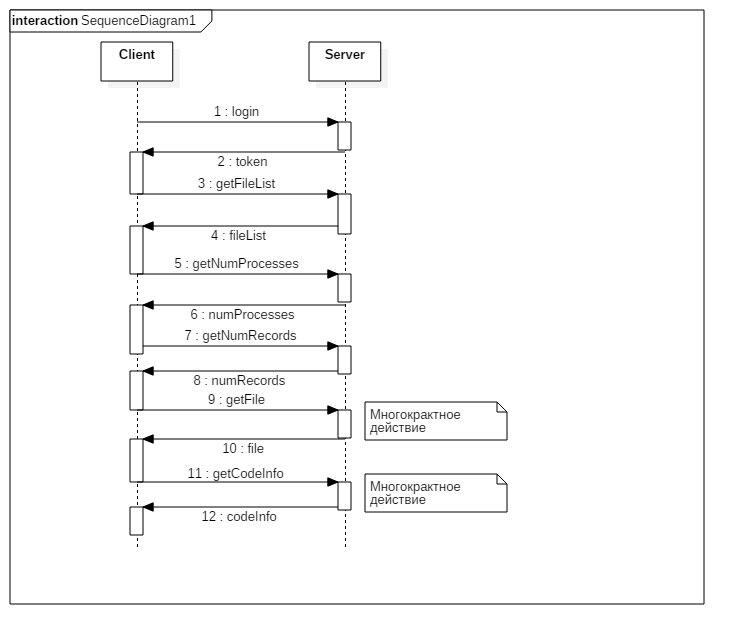
\includegraphics[width=1.1\textwidth]{img/clientServer.jpg}
	\caption{Диаграмма взамодействия клиента и сервера}
	\label{fig:spire12}
\end{figure}
В начале работы приложения клиент должен пройти авторизацию(1). В случае успешного прохождения авторизации ему посылается token,позволяющий ему получить права доступа к работе с trace-информацией(2). После этого клиент загружает список доступных ему файлов(3-4).
Запросы (5-8) технические и нужны для корректного отображения trace-информации на стороне клиента.  После того как вся техническая информация была загружена, клиент приступает к загрузке файла(9-10). Файл загружается <<небольшими порциями>>, поэтому возможно многократное повторение запросов (9-10) до успешной загрузки файла. В случае успешной загрузки файла клиент может получить детальную информацию об этом файле при помоще запросов (11-12).
\section{Синтаксический анализ trace-файлов}
Для синтаксического анализа(парсинга) trace-файлов и занесения их в базу данных была разработана консольная программа.
\begin{figure}[h!]
	\centering
	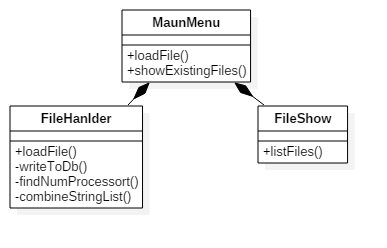
\includegraphics[width=0.6\textwidth]{img/server.png}
	\caption{Диаграмма классов серверного приложения}
	\label{fig:spire11}
\end{figure}
\\ \textbf{MainMenu.} Класс главного меню программы. Реализует логику взаимодействия между клиентом и программов. \\
\textbf{FileShow.} Класс для работы с файловой системой компьютера. \\
\textbf{FileHandler.} Класс для парсинга trace-файла. Реализует логику анализа trace-файла и занесения его в базу данных.
\section{Базы данных}
Для хранения файлов трасс формата PICL была спроектирована база данных.
\begin{lstlisting}[language=SQL]
CREATE TABLE Tracks ( 
filename VARCHAR(50) NOT NULL,
typeRecord INT NOT NULL,
typeEvent INT NOT NULL,
time FLOAT NOT NULL,
prid INT NOT NULL,
pid INT NOT NULL,
numData INT NOT NULL,
data VARCHAR(200),
FOREIGN KEY (typeEvent) REFERENCES Codes(code) 
ON DELETE CASCADE ON UPDATE CASCADE,
FOREIGN KEY (filename) REFERENCES Files(filename) 
ON DELETE CASCADE ON UPDATE CASCADE
) ENGINE = INNODB DEFAULT CHARSET=utf8;
\end{lstlisting}
Так же были спроектированы вспомогательные базы данных для хранения информации о событиях MPI, файлах, пользователях.
\begin{figure}[h!]
	\centering
	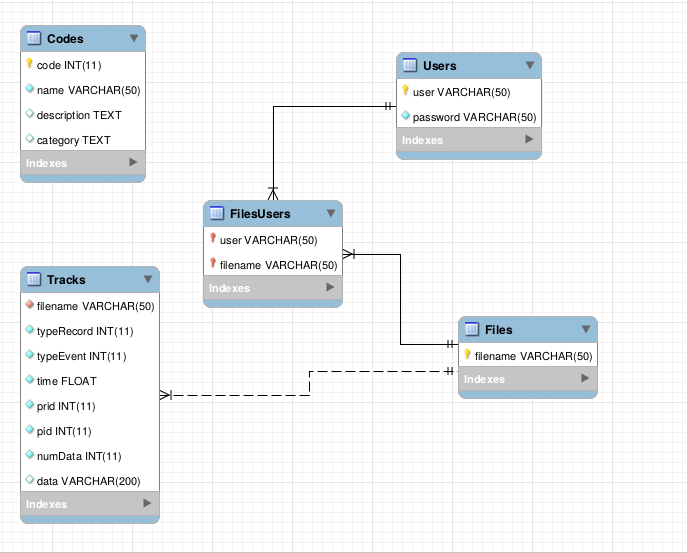
\includegraphics[width=0.8\textwidth]{img/img7.png}
	\caption{Диаграмма классов серверного приложения}
	\label{fig:spire12}
\end{figure}

\begin{lstlisting}[language=SQL]
CREATE TABLE Users(
user  VARCHAR(50) NOT NULL  PRIMARY KEY,
password  VARCHAR(50) NOT NULL
) ENGINE = INNODB DEFAULT CHARSET=utf8;

CREATE TABLE Files(
filename  VARCHAR(50) NOT NULL PRIMARY KEY
) ENGINE = INNODB DEFAULT CHARSET=utf8;

CREATE TABLE FilesUsers(
user  VARCHAR(50) NOT NULL,
filename  VARCHAR(50) NOT NULL,
PRIMARY KEY (user, filename), 
FOREIGN KEY (filename) REFERENCES Files(filename)
ON DELETE CASCADE ON UPDATE CASCADE 
) ENGINE = INNODB DEFAULT CHARSET=utf8;

CREATE TABLE Codes(
code  INT NOT NULL  PRIMARY KEY,
name  VARCHAR(50) NOT NULL,
description TEXT,
category TEXT
) ENGINE = INNODB DEFAULT CHARSET=utf8;

\end{lstlisting} 

\subsection{Нормальные формы}
Нормальная форма — свойство отношения в реляционной модели данных, характеризующее его с точки зрения избыточности, потенциально приводящей к логически ошибочным результатам выборки или изменения данных. Нормальная форма определяется как совокупность требований, которым должно удовлетворять отношение.
Процесс преобразования отношений базы данных (БД) к виду, отвечающему нормальным формам, называется нормализацией. Нормализация предназначена для приведения структуры БД к виду, обеспечивающему минимальную логическую избыточность, и не имеет целью уменьшение или увеличение производительности работы или же уменьшение или увеличение физического объёма базы данных. Конечной целью нормализации является уменьшение потенциальной противоречивости хранимой в базе данных информации. Как отмечает К. Дейт, общее назначение процесса нормализации заключается в следующем:
\begin{enumerate}

	\item исключение некоторых типов избыточности;
	\item устранение некоторых аномалий обновления;
	\item разработка проекта базы данных, который является достаточно «качественным» представлением реального мира, интуитивно понятен и может служить хорошей основой для последующего расширения;
	\item упрощение процедуры применения необходимых ограничений целостности.

\end{enumerate}
Устранение избыточности производится, как правило, за счёт декомпозиции отношений таким образом, чтобы в каждом отношении хранились только первичные факты (то есть факты, не выводимые из других хранимых фактов)\cite{book6}.

\textbf{Первая нормальная форма}. Переменная отношения находится в первой нормальной форме тогда и только тогда, когда в любом допустимом значении отношения каждый его кортеж содержит только одно значение для каждого из атрибутов.
В реляционной модели отношение всегда находится в первой нормальной форме по определению понятия отношение.
Что же касается различных таблиц, то они могут не быть правильными представлениями отношений и, соответственно, могут не находиться в 1NF. В соответствии с определением К. Дж. Дейта для такого случая, таблица нормализована (эквивалентно — находится в первой нормальной форме) тогда и только тогда, когда она является прямым и верным представлением некоторого отношения. Конкретнее, рассматриваемая таблица должна удовлетворять следующим пяти условиям:
\begin{enumerate}
\item Нет упорядочивания строк сверху-вниз (другими словами, порядок строк не несет в себе никакой информации).
\item Нет упорядочивания столбцов слева-направо (другими словами, порядок столбцов не несет в себе никакой информации).
\item Нет повторяющихся строк.
\item Каждое пересечение строки и столбца содержит ровно одно значение из соответствующего домена.
\item Все столбцы являются обычными (в таблице нет «скрытых» компонентов, которые могут быть доступны только в вызове некоторого специального оператора взамен ссылок на имена регулярных столбцов).
\end{enumerate}
В моей базе данных каждый кортеж всех таблиц содержит только атомарные атрибуты (атрибут атомарен, если его значение теряет смысл при любом разбиении на части или переупорядочивании), отсутствуют повторяющиеся кортежи. Исходя из этого, можно сказать, что все таблицы находятся в первой нормальной форме.

\textbf{Вторая нормальная форма}. Переменная отношения находится во второй нормальной форме тогда и только тогда, когда она находится в первой нормальной форме и каждый неключевой атрибут неприводимо зависит от её потенциального ключа.
Неприводимость означает, что в составе потенциального ключа отсутствует меньшее подмножество атрибутов, от которого можно также вывести данную функциональную зависимость. Для неприводимой функциональной зависимости часто используется эквивалентное понятие «полная функциональная зависимость». Если потенциальный ключ является простым, то есть состоит из единственного атрибута, то любая функциональная зависимость от него является неприводимой (полной). Если потенциальный ключ является составным, то согласно определению второй нормальной формы в отношении не должно быть неключевых атрибутов, зависящих от части составного потенциального ключа.
Вторая нормальная форма по определению запрещает наличие неключевых атрибутов, которые вообще не зависят от потенциального ключа. Таким образом, вторая нормальная форма запрещает создавать отношения как несвязанные (хаотические, случайные) наборы атрибутов.
В моей базе данных не все потенциальные ключи состоят из одного атрибута, следовательно, нельзя сказать, что все таблицы находятся во второй нормальной форме.

%%% Local Variables:

%%% mode: latex
%%% TeX-master: "rpz"
%%% End:
%--количество цветов
%||количество пикселей